% Shared style and exact pattern-block geometry. Compile with pdfLaTeX.
\usepackage[letterpaper,margin=0.65in,top=0.60in,bottom=0.65in]{geometry}
\usepackage[T1]{fontenc}
\usepackage[default]{sourcesanspro}
\usepackage{microtype,tikz,array,tabularx,fancyhdr}
\usepackage[hidelinks]{hyperref}
\usetikzlibrary{calc}
\setlength{\parindent}{0pt}
\setlength{\parskip}{7pt}
\setlength{\headheight}{0pt}
\setlength{\footskip}{26pt}
\setlength{\emergencystretch}{2em}
\pagestyle{fancy}\fancyhf{}
\renewcommand{\headrulewidth}{0pt}
\renewcommand{\footrulewidth}{0.4pt}
\fancyfoot[L]{\scriptsize Bellingham Math Circle\enspace /\enspace Week 1\enspace /\enspace \activityid}
\fancyfoot[R]{\scriptsize \thepage}
\definecolor{ink}{gray}{0.12}
\definecolor{soft}{gray}{0.95}
\color{ink}
\newlength{\blockside}
\setlength{\blockside}{1in} % Change here if your blocks have another edge length.
\def\hh{0.8660254037844386}
\tikzset{outline/.style={draw=ink,line width=1.1pt,line join=round},
  tile/.style={draw=ink,line width=0.65pt,line join=round,fill=white},
  tilelabel/.style={font=\bfseries\small,inner sep=1pt}}
\newcommand{\HexPath}{(-1,0)--(-.5,-\hh)--(.5,-\hh)--(1,0)--(.5,\hh)--(-.5,\hh)--cycle}
\newcommand{\PennantPath}{(-1,0)--(-.5,-\hh)--(.5,-\hh)--(1,0)--(.5,\hh)--(0,2*\hh)--(-.5,\hh)--cycle}
\newcommand{\DoublePath}{(-1,0)--(-.5,-\hh)--(.5,-\hh)--(1,0)--(.5,\hh)--(1,2*\hh)--(.5,3*\hh)--(-.5,3*\hh)--(-1,2*\hh)--(-.5,\hh)--cycle}
\newcommand{\BluePath}{(-.75,-.5*\hh)--(.25,-.5*\hh)--(.75,.5*\hh)--(-.25,.5*\hh)--cycle}
\newcommand{\RedPath}{(-1,-.5*\hh)--(1,-.5*\hh)--(.5,.5*\hh)--(-.5,.5*\hh)--cycle}
\newcommand{\DrawOutline}[1]{\begin{tikzpicture}[x=\blockside,y=\blockside]\draw[outline] #1;\end{tikzpicture}}
\newcommand{\PageTitle}[2]{
  {\fontsize{10}{12}\selectfont\bfseries WEEK 1\quad PATTERN BLOCKS\hfill #1\par}
  \vspace{3pt}{\fontsize{27}{30}\selectfont\bfseries #2\par}\vspace{2pt}}
\newcommand{\NameLine}{{\small Name: \rule{2.65in}{.4pt}\hfill Date: \rule{1.35in}{.4pt}\par}\vspace{4pt}}
\newcommand{\Task}[2]{\par\vspace{3pt}{\large\bfseries #1}\par #2\par}
\newcommand{\RuleBox}[1]{\par\begingroup\setlength{\fboxsep}{8pt}\colorbox{soft}{\parbox{\dimexpr\linewidth-16pt\relax}{#1}}\endgroup\par}
\newcommand{\WriteBox}[2]{\par\textbf{#1}\par\vspace{2pt}\begin{tikzpicture}\draw[draw=black!40,line width=.5pt] (0,0) rectangle (\dimexpr\linewidth-.5pt\relax,#2);\end{tikzpicture}\par}
\newcommand{\Pair}[1]{
  \par\vspace{3pt}\noindent
  \begin{minipage}[t]{.485\linewidth}\centering\textbf{Copy A}\par\vspace{8pt}\DrawOutline{#1}\end{minipage}\hfill
  \begin{minipage}[t]{.485\linewidth}\centering\textbf{Copy B}\par\vspace{8pt}\DrawOutline{#1}\end{minipage}\par\vspace{4pt}}
\newcommand{\ColorLists}{\begin{tabularx}{\linewidth}{@{}X X@{}}
  Colors in A: \hrulefill & Colors in B: \hrulefill
  \end{tabularx}\par}
\newcommand{\PieceCounts}{\begin{tabularx}{\linewidth}{@{}X X X@{}}
  Pieces in A: \hrulefill & Pieces in B: \hrulefill & Total: \hrulefill
  \end{tabularx}\par}
\newcommand{\ScaleCheck}{\vfill\par\begingroup\fontsize{9}{11}\selectfont
  \begin{minipage}[c]{1.2in}\centering
  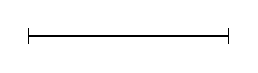
\begin{tikzpicture}[x=\blockside,y=1in]\draw[line width=.65pt] (0,0)--(1,0);\draw (0,-.04)--(0,.04) (1,-.04)--(1,.04);\end{tikzpicture}\par
  One block edge
  \end{minipage}\hfill
  \begin{minipage}[c]{\dimexpr\linewidth-1.35in\relax}
  Adult: print at \textbf{100\% / Actual Size}, single-sided. This line is 1 inch (25.4 mm) in the default file. Match a green triangle's edge to it before using the mats.
  \end{minipage}\par\endgroup}
\newcommand{\StudentFooter}{\vfill{\small Build first. You may explain by pointing, talking, or drawing.}\par}
\newcommand{\Allowed}{{\small Use only green triangles, blue rhombi, red trapezoids, and yellow hexagons.\par}}
\newcommand{\CoverRule}{Cover each outline exactly: no gaps, overlaps, or pieces outside.}
\newcommand{\ColorRule}{Keep both copies built. A color used in A cannot be used in B.}
% Small labeled diagrams for adult solutions only; these are not actual-size mats.
\newcommand{\Tile}[3]{\path[tile] #1;\node[tilelabel] at #2 {#3};}
\newcommand{\PoneYG}{
 \Tile{\HexPath}{(0,0)}{Y}
 \Tile{(-.5,\hh)--(.5,\hh)--(0,2*\hh)--cycle}{(0,1.3333*\hh)}{G}}
\newcommand{\PoneRBB}{
 \Tile{(0,0)--(.5,\hh)--(0,2*\hh)--(-.5,\hh)--cycle}{(0,\hh)}{B}
 \Tile{(0,0)--(.5,-\hh)--(1,0)--(.5,\hh)--cycle}{(.5,0)}{B}
 \Tile{(-.5,\hh)--(-1,0)--(-.5,-\hh)--(.5,-\hh)--cycle}{(-.4,-.3*\hh)}{R}}
\newcommand{\HexReds}{
 \Tile{(-1,0)--(1,0)--(.5,\hh)--(-.5,\hh)--cycle}{(0,.43*\hh)}{R}
 \Tile{(-1,0)--(-.5,-\hh)--(.5,-\hh)--(1,0)--cycle}{(0,-.43*\hh)}{R}}
\newcommand{\HexBlues}{
 \Tile{(0,0)--(1,0)--(.5,\hh)--(-.5,\hh)--cycle}{(.25,.5*\hh)}{B}
 \Tile{(0,0)--(-.5,\hh)--(-1,0)--(-.5,-\hh)--cycle}{(-.5,0)}{B}
 \Tile{(0,0)--(-.5,-\hh)--(.5,-\hh)--(1,0)--cycle}{(.25,-.5*\hh)}{B}}
\newcommand{\DoubleTiles}[1]{#1\begin{scope}[shift={(0,2*\hh)}]#1\end{scope}}
\newcommand{\SolutionPic}[1]{\begin{tikzpicture}[x=.54in,y=.54in]#1\end{tikzpicture}}
